\documentclass[aspectratio=169,10pt,t]{beamer}
\usepackage{issa}  % place issa.sty in the same folder
\definecolor{AccentCol}{HTML}{9B5E1A}
\renewcommand{\lecnum}{8}
\begin{document}
\titleslide{8}{Reinforcement Learning Part 3:\\Multi-Agent Systems \& Autonomous Combat Platforms}{MARL \textbullet\ CTDE \textbullet\ QMIX \textbullet\ MAPPO \textbullet\ MADDPG \textbullet\ credit assignment \textbullet\ emergent tactics\\Case study: 6-unit combined arms (3 ground + 2 drones + 1 SEAD) --- emergent flanking and decoy tactics}

\sect{1. Why MARL}
\begin{frame}{Why Multi-Agent RL? --- The Limits of Single-Agent Approaches}
\begin{columns}[T]
\column{0.52\textwidth}
\begin{cbox}[ISSAred]{What a single agent cannot model}\scriptsize
\textbf{\textcircled{\tiny1} Simultaneous actors:} 6 units act concurrently; each action affects everyone's reward; one agent controls one entity.\\
\textbf{\textcircled{\tiny2} Partial observability per unit:} a drone sees 200 m, a tank 500 m; nobody has the full picture.\\
\textbf{\textcircled{\tiny3} Cooperative reward:} mission success is a JOINT outcome; individual credit is ambiguous.\\
\textbf{\textcircled{\tiny4} Emergent tactics:} flanking needs unit A to distract while B moves.\\
\textbf{\textcircled{\tiny5} Adversarial dynamics:} OPFOR is also multi-agent and adapts --- the environment is non-stationary.\end{cbox}
\column{0.46\textwidth}
\figc{3.3cm}{\begin{tikzpicture}[x=0.55cm,y=0.55cm]
\draw[ISSAgrey,fill=ISSAgrn!5](0,0)rectangle(9,6);
\foreach \x/\y/\r/\l in {1.5/1.5/1.8/ARM,1.5/3.5/1.1/INF,6.0/4.6/0.7/ISR}{\draw[AccentCol!60,dashed](\x,\y)circle(\r);\node[circle,fill=AccentCol,inner sep=1.5pt]at(\x,\y){};\node[font=\tiny,anchor=north]at(\x,\y-0.1){\l};}
\foreach \x/\y in {7.4/1.6,8.0/2.4}{\node[circle,fill=ISSAred,inner sep=1.6pt]at(\x,\y){};}\node[font=\tiny,ISSAred]at(7.7,0.9){OPFOR};
\node[lab]at(4.5,-0.5){dashed circles: each unit's own sensor range};
\end{tikzpicture}}
\begin{ibox}\scriptsize No unit sees the whole battlefield, and none can win alone --- the defining features of a multi-agent problem.\end{ibox}
\end{columns}
\end{frame}

\begin{frame}{The MARL Paradigm --- $N$ Learning Agents in One Shared World}
\begin{columns}[T]
\column{0.50\textwidth}
\begin{fbx}{Dec-POMDP}\[\big(S,\{A_i\},P,\{r_i\},\{\Omega_i\},O,\gamma\big)\]\[\pi_{\theta_i}(a_i|o_i),\quad \mathbf a=(a_1,\ldots,a_N),\quad r(s,\mathbf a)\text{ or }r_i(s,\mathbf a)\]\end{fbx}
\begin{wbox}\scriptsize\textbf{Fundamental challenge --- non-stationarity:} from agent $i$'s view, the other $N-1$ agents are part of the environment AND they are learning. The ``environment'' keeps changing even with fixed physics, so single-agent convergence theorems no longer apply.\end{wbox}
\column{0.48\textwidth}
\figc{2.4cm}{\begin{tikzpicture}
\tikzset{S/.style={nd,text width=2.0cm,minimum height=1.3cm,font=\fontsize{6.2}{7.2}\selectfont}}
\node[S,fill=ISSAgrn!12,draw=ISSAgrn](a)at(0,0){\textbf{Fully cooperative}\\shared reward $r_i=r$\\combined-arms attack};
\node[S,fill=ISSAred!10,draw=ISSAred](b)at(2.35,0){\textbf{Fully competitive}\\zero-sum\\Blue vs Red};
\node[S,fill=AccentCol!15,draw=AccentCol](c)at(4.7,0){\textbf{Mixed}\\cooperative Blue team vs Red team};
\node[lab]at(4.7,-0.9){most real military scenarios};
\end{tikzpicture}}
\begin{rbox}\scriptsize\textbf{The mark of modern warfare:} unmanned systems fighting in coordinated swarms, autonomous wingmen, manned--unmanned teams --- all multi-agent problems.\end{rbox}
\end{columns}
\end{frame}

\sect{2. CTDE}
\begin{frame}{CTDE --- Centralised Training, Decentralised Execution}
\figc{2.7cm}{\begin{tikzpicture}
\begin{scope}\node[font=\scriptsize\bfseries,AccentCol]at(2.2,1.9){TRAINING (simulation)};\node[ndN,minimum width=3.6cm,minimum height=0.7cm](cr)at(2.2,1.2){centralised critic / mixer: sees global state $s$};\foreach \i in {1,2,3}{\node[ndA,minimum width=1.1cm](a\i)at(\i*1.3-0.4,0){actor \i};\draw[arr,<->](a\i)--(cr);}\end{scope}
\draw[bigarr](5.0,0.6)--(6.6,0.6)node[midway,above,font=\tiny]{deploy actors only};
\begin{scope}[xshift=7.4cm]\node[font=\scriptsize\bfseries,AccentCol]at(2.2,1.9){EXECUTION (field)};\foreach \i in {1,2,3}{\node[ndA,minimum width=1.1cm](b\i)at(\i*1.3-0.4,0){actor \i};\node[nds](o\i)at(\i*1.3-0.4,1.0){$o_\i$};\draw[arr](o\i)--(b\i);}\node[font=\tiny,ISSAred]at(2.2,-0.65){radio silence: no critic, no comms needed};\end{scope}
\end{tikzpicture}}
\begin{columns}[T]
\column{0.50\textwidth}
\begin{tl}\item \textbf{Training:} use GLOBAL information (all observations, actions, full state) to train a centralised critic/mixer $\Rightarrow$ better credit assignment; coordination emerges\item \textbf{Execution:} each agent acts on its OWN local observation $o_i$ $\Rightarrow$ no bandwidth needed, works even when comms are jammed\end{tl}
\begin{fbx}{Decomposition}\[\text{actor: }\pi_i(a_i|o_i;\theta_i)\quad\text{critic: }V(s,o_{1..N},a_{1..N};\phi)\]\end{fbx}
\column{0.48\textwidth}
\begin{rbox}\scriptsize\textbf{Military analogy:} the commander briefs each unit on the plan (centralised), then radio silence --- units execute independently on what they see (decentralised). This is mission command: shared intent, local initiative.\end{rbox}
\end{columns}
\end{frame}

\begin{frame}{Three CTDE Algorithms --- QMIX, MAPPO and MADDPG}
\figc{4.7cm}{\begin{tikzpicture}
\tikzset{C/.style={nd,text width=4.6cm,align=left,minimum height=4.3cm,font=\fontsize{6.6}{7.9}\selectfont,inner sep=3pt,anchor=north}}
\node[C,draw=ISSAblue,fill=ISSAblue!6]at(-4.9,0){\textbf{\textcolor{ISSAblue}{QMIX (Rashid 2018) --- value-based}}\\[2pt]Each agent has a local $Q_i(o_i,a_i)$. A mixer combines them: $Q_{\text{tot}}=f(Q_1,\ldots,Q_N;s)$.\\[2pt]\textbf{Key constraint --- monotonicity:} $\partial Q_{\text{tot}}/\partial Q_i>0$ (positive weights) $\Rightarrow$ the joint argmax equals the per-agent argmaxes $\Rightarrow$ decentralised execution guaranteed.\\[2pt]Training: TD loss on $Q_{\text{tot}}$ against $r+\gamma Q_{\text{tot}}^{\text{target}}$.};
\node[C,draw=AccentCol,fill=AccentCol!8]at(0,0){\textbf{\textcolor{AccentCol}{MAPPO (Yu 2022) --- policy gradient}}\\[2pt]Extends PPO to $N$ agents with \textbf{parameter sharing} across agents.\\[2pt]Centralised critic $V(s)$ on the full global state; each agent's PPO update uses $V(s)$ as baseline.\\[2pt]Works well when agents are homogeneous; sharing dramatically reduces parameter count.};
\node[C,draw=ISSAred,fill=ISSAred!5]at(4.9,0){\textbf{\textcolor{ISSAred}{MADDPG (Lowe 2017) --- actor--critic}}\\[2pt]Deterministic actors $a_i=\mu_i(o_i;\theta_i)$.\\[2pt]Each agent has its OWN centralised critic $Q_i(s,a_1,\ldots,a_N;\phi_i)$ that sees every agent's action.\\[2pt]Suits continuous actions and mixed cooperative--competitive settings (each agent can have its own reward).};
\end{tikzpicture}}
\end{frame}

\sect{3. QMIX}
\begin{frame}{QMIX --- Global $Q$ as a Monotonic Mix of Local $Q$-Values}
\begin{columns}[T]
\column{0.52\textwidth}
\figc{3.2cm}{\begin{tikzpicture}
\foreach \i in {1,2,3}{\node[nds](o\i)at(\i*1.6-1.6,0){$o_\i,a_\i^{\text{prev}}$};\node[ndA,minimum width=1.3cm](q\i)at(\i*1.6-1.6,1.0){GRU agent\\$Q_\i(o_\i,\cdot)$};\draw[arr](o\i)--(q\i);}
\node[ndN,minimum width=4.4cm,minimum height=0.8cm](mx)at(1.6,2.4){mixer: $Q_{\text{tot}}=W_2\,\text{ELU}(W_1[Q_1..Q_N]+b_1)+b_2$};
\foreach \i in {1,2,3}{\draw[arr](q\i)--(mx);}
\node[ndY](hn)at(5.5,2.4){hypernet\\$s\to|W_1|,|W_2|$};\draw[arr](hn)--(mx);\node[nds](s)at(5.5,1.1){global state $s$};\draw[arr](s)--(hn);
\end{tikzpicture}}
\begin{tl}\item Agent networks: one per agent, shared weights; a GRU handles partial observability\item The hypernetwork maps $s$ to mixing weights, made positive with absolute values; biases may take any sign\end{tl}
\column{0.46\textwidth}
\begin{fbx}{Monotonicity $\Rightarrow$ decentralised greedy execution}\[\frac{\partial Q_{\text{tot}}}{\partial Q_i}>0\ \Rightarrow\]\[\arg\max_{\mathbf a}Q_{\text{tot}}=\big(\arg\max_{a_1}Q_1,\ldots,\arg\max_{a_N}Q_N\big)\]\end{fbx}
\begin{rbox}\scriptsize\textbf{Each agent independently picks ITS best action} --- and the team's joint choice is still optimal for $Q_{\text{tot}}$. No negotiation needed at execution time.\end{rbox}
\begin{wbox}\scriptsize\textbf{Limitation:} monotonic mixing cannot represent situations where one agent's best action depends on another's (e.g.\ ``only advance if the other unit holds''). Richer coordination needs other methods.\end{wbox}
\end{columns}
\end{frame}

\begin{frame}{QMIX Case Study --- Combined Arms with 6 Agents}
\begin{columns}[T]
\column{0.50\textwidth}
\begin{cbox}[ISSAnavy]{Environment}\scriptsize 3 ground units (infantry, armour, artillery) + 2 ISR drones + 1 SEAD aircraft. Objective: destroy a defended position held by 2 SAM sites and 4 OPFOR infantry. Observation per agent (42-D): own position, health, ammo, role; visible units in sensor range; friendly positions if comms are not jammed. QMIX state = 6 $\times$ 42 = 252-D.\end{cbox}
\figc{2.2cm}{\bars{100}{1.5}{2.1}{Mission success (\%)/74.1/AccentCol,OPFOR neutralised (of 6 $\times$ 16.7)/86.7/ISSAgrn}}
\sm{QMIX after 200K episodes: success 74.1\%; 38.2 turns per episode; 1.8 friendly casualties; 5.2/6 targets neutralised; $\sim$18 h on 8 CPU workers.}
\column{0.48\textwidth}
\begin{rbox}\scriptsize\textbf{Emergent behaviour:} the SEAD aircraft ALWAYS neutralises the SAM sites first, and ground units converge only after the SAMs are down. The agents discovered suppression-then-advance --- standard SEAD doctrine --- from reward alone.\end{rbox}
\figc{2.3cm}{\begin{tikzpicture}\draw[->](0,0)--(6,0)node[right,font=\tiny]{time};
\node[ndR,minimum width=1.6cm](a)at(1.0,0.6){SEAD hits SAM};\node[ndA,minimum width=1.6cm](b)at(3.0,0.6){ISR overwatch};\node[ndG,minimum width=1.6cm](c)at(5.0,0.6){ground advance};\draw[arr](a)--(b);\draw[arr](b)--(c);
\node[lab]at(3,-0.35){learned sequence: suppress, observe, then advance};\end{tikzpicture}}
\end{columns}
\end{frame}

\sect{4. MAPPO}
\begin{frame}{MAPPO --- Multi-Agent PPO with a Shared Centralised Critic}
\begin{columns}[T]
\column{0.52\textwidth}
\begin{cbox}{Four design choices}\scriptsize \textbf{\textcircled{\tiny1} Shared actor parameters:} all agents use one network $\pi(a_i|o_i;\theta)$ with agent ID one-hot in the input: 6 agents $\to$ 1 actor ($N\times$ efficiency).\\ \textbf{\textcircled{\tiny2} Centralised critic:} $V(s;\phi)$ on the global state, one critic for all; $\hat A_i=r+\gamma V(s')-V(s)$.\\ \textbf{\textcircled{\tiny3} PPO clipping per agent:} $L_i^{\text{CLIP}}$ with $r_i(\theta)=\pi_i^{\text{new}}/\pi_i^{\text{old}}$.\\ \textbf{\textcircled{\tiny4} Advantage normalisation:} $\hat A_i\leftarrow(\hat A_i-\text{mean})/(\text{std}+\epsilon)$ across agents and steps --- critical for stability.\end{cbox}
\begin{fbx}{MAPPO loss}\[L=\frac1N\sum_iL_i^{\text{CLIP}}(\theta)+c_1L_{\text{critic}}(\phi)-c_2H(\pi_i)\]\end{fbx}
\column{0.46\textwidth}
\figc{2.6cm}{\begin{tikzpicture}
\node[ndA,minimum width=3.4cm](ac)at(0,0){one shared actor $\theta$};\foreach \i/\l in {1/INF,2/ARM,3/ART,4/ISR1,5/ISR2,6/SEAD}{\node[nds,minimum width=0.75cm,inner sep=1pt](u\i)at(\i*0.82-2.87,-1.1){\l};\draw[arr](ac)--(u\i);}
\node[ndN,minimum width=3.4cm](cr)at(0,1.1){centralised critic $V(s;\phi)$};\draw[arr](cr)--(ac);
\end{tikzpicture}}
\begin{ibox}\scriptsize Parameter sharing means every unit's experience trains the same network: the infantry agent benefits from what the armour agent learned, as units share lessons in an after-action review.\end{ibox}
\end{columns}
\end{frame}

\begin{frame}{MAPPO vs QMIX --- and the Human-Expert Benchmark}
\begin{columns}[T]
\column{0.48\textwidth}
\figc{1.9cm}{\scriptsize\renewcommand{\arraystretch}{1.12}\begin{tabular}{ll}\toprule\textbf{QMIX}&\textbf{MAPPO}\\\midrule monotonic coordination guarantee&PPO clipping: robust\\off-policy (replay, sample-efficient)&on-policy (fresh data)\\purely cooperative (shared reward)&mixed coop.--competitive\\homogeneous obs.\ preferred&heterogeneous agents OK\\\bottomrule\end{tabular}}
\subhead{Combined-arms results}
\figc{2.6cm}{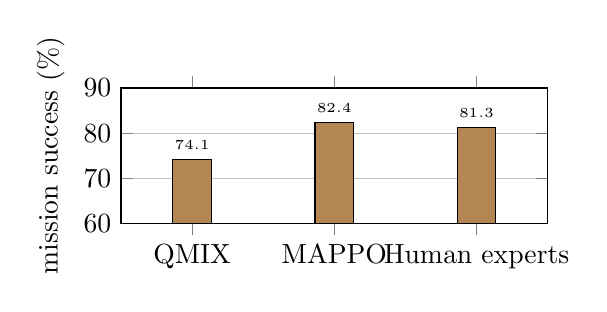
\begin{tikzpicture}\begin{axis}[ybar,width=7.0cm,height=3.3cm,symbolic x coords={QMIX,MAPPO,Human experts},xtick=data,ymin=60,ymax=90,bar width=14pt,enlarge x limits=0.25,ylabel={mission success (\%)},nodes near coords,nodes near coords style={font=\fontsize{5.5}{6}\selectfont},ymajorgrids]
\addplot[fill=AccentCol!75]coordinates{(QMIX,74.1)(MAPPO,82.4)(Human experts,81.3)};
\end{axis}\end{tikzpicture}}
\column{0.50\textwidth}
\begin{rbox}\scriptsize\textbf{MAPPO:} mission success \textbf{82.4\%} (best no-comms MARL result); 33.7 turns per episode (faster than QMIX); 1.2 casualties per mission; 5.7/6 targets neutralised.\end{rbox}
\begin{cbox}[ISSAnavy]{Human-expert team benchmark}\scriptsize 3 experienced military planners, same scenario, manual decisions each turn: \textbf{81.3\%} success, 41.8 turns, 1.6 casualties. \textbf{MAPPO slightly exceeds the human team} --- in this simulation.\end{cbox}
\begin{wbox}\scriptsize 82.4\% vs 81.3\% is a 1.1-point gap: without the number of evaluation episodes and a confidence interval we cannot call it a real difference (Section 0 of Lecture 1). The honest claim is ``comparable to experts''.\end{wbox}
\end{columns}
\end{frame}

\sect{5. Credit Assignment}
\begin{frame}{Credit Assignment --- Who Deserves Credit for a Joint Victory?}
\begin{columns}[T]
\column{0.50\textwidth}
\begin{cbox}[ISSAnavy]{Mission succeeds (+100). Who earned it?}\scriptsize Agent 1 infantry: suppressive fire. Agent 2 armour: advanced under cover. Agent 3 artillery: fired too early --- missed. Agent 4 drone 1: ISR (critical). Agent 5 drone 2: malfunctioned, did nothing. Agent 6 SEAD: neutralised the SAM (critical).\end{cbox}
\begin{wbox}\scriptsize\textbf{Naive split:} every agent gets $100/6=+16.7$ --- the artillery that missed and the drone that did nothing are REWARDED. Agents learn ``do nothing, still win'': the \textbf{free-rider problem}.\end{wbox}
\column{0.48\textwidth}
\figc{2.8cm}{\begin{tikzpicture}\begin{axis}[ybar,width=6.8cm,height=3.5cm,symbolic x coords={INF,ARM,ART,ISR1,ISR2,SEAD},xtick=data,ymin=0,ymax=20,bar width=10pt,ylabel={reward},nodes near coords,nodes near coords style={font=\fontsize{5}{6}\selectfont},ymajorgrids,title={naive equal split}]
\addplot[fill=ISSAgrey!70]coordinates{(INF,16.7)(ARM,16.7)(ART,16.7)(ISR1,16.7)(ISR2,16.7)(SEAD,16.7)};
\end{axis}\end{tikzpicture}}
\begin{ibox}\scriptsize\textbf{QMIX's partial answer:} the factorisation gives each agent its own $Q_i$; an idle agent's $Q_5\approx0$, and the mixer weights contributions by the global state.\end{ibox}
\end{columns}
\end{frame}

\begin{frame}{COMA --- Counterfactual Credit: ``What If Only I Had Acted Differently?''}
\begin{columns}[T]
\column{0.50\textwidth}
\begin{fbx}{Counterfactual baseline (Foerster 2018)}\[b_i(s,\mathbf a_{-i})=\sum_{a_i'}\pi_i(a_i'|o_i)\,Q\big(s,(a_i',\mathbf a_{-i})\big)\]\[A_i(s,\mathbf a)=Q(s,\mathbf a)-b_i(s,\mathbf a_{-i})\]\end{fbx}
\begin{tl}\item Centralised critic $Q(s,a_1,\ldots,a_N)$\item ``What would the team's value be if everyone else did the same but agent $i$ acted on average?''\item $A_i$ = how much $a_i$ improved over agent $i$'s own average\end{tl}
\column{0.48\textwidth}
\figc{3.0cm}{\begin{tikzpicture}\begin{axis}[ybar,width=6.8cm,height=3.7cm,symbolic x coords={INF,ARM,ART,ISR1,ISR2,SEAD},xtick=data,ymin=-5,ymax=14,bar width=10pt,ylabel={COMA advantage $A_i$},nodes near coords,nodes near coords style={font=\fontsize{5}{6}\selectfont},ymajorgrids]
\addplot[fill=ISSAgrn!70]coordinates{(INF,8.4)(ARM,12.1)(ISR1,9.8)(SEAD,11.4)};\addplot[fill=ISSAred!70,bar shift=0pt]coordinates{(ART,-3.2)(ISR2,-1.1)};
\end{axis}\end{tikzpicture}}
\begin{rbox}\scriptsize The missed artillery shot ($-3.2$) and the idle drone ($-1.1$) are correctly penalised; armour (+12.1), SEAD (+11.4) and ISR (+9.8) earn the most credit.\end{rbox}
\sm{The PPTX states that the advantages sum to $\approx0$ (a baseline property); the six values shown sum to $+37.4$, so that claim does not hold for this table.}
\end{columns}
\end{frame}

\sect{6. Emergent Behaviour}
\begin{frame}{Emergent Communication --- Agents Invent a Language}
\begin{columns}[T]
\column{0.50\textwidth}
\begin{cbox}{Set-up}\scriptsize Add a channel: each agent broadcasts a message $m_i\in\mathbb{R}^{8}$ (a learned ``language''). Actor input: $[o_i,m_1,\ldots,m_{N-1}]$. Agents learn both WHAT to broadcast and how to USE others' messages --- purely by gradient descent.\end{cbox}
\figc{2.0cm}{\begin{tikzpicture}[x=0.75cm]
\foreach \i in {0,...,7}{\pgfmathsetmacro{\cl}{ifthenelse(\i<3,1,ifthenelse(\i<6,2,3))}\fill[\ifnum\i<3 ISSAblue!50\else\ifnum\i<6 ISSAred!50\else ISSAamb!60\fi\fi](\i,0)rectangle++(0.95,0.6);\node[font=\tiny]at(\i+0.47,0.3){$m_\i$};}
\node[font=\tiny,ISSAblue,anchor=north]at(1.5,-0.05){enemy position};\node[font=\tiny,ISSAred,anchor=north]at(4.5,-0.05){SAM lock-on status};\node[font=\tiny,ISSAamb!70!black,anchor=north]at(7,-0.05){own fuel};
\end{tikzpicture}}
\sm{Linear-probe analysis of drone messages after 50K training episodes.}
\column{0.48\textwidth}
\figc{2.4cm}{\bars{100}{1.7}{2.1}{MAPPO without comms/82.4/ISSAgrey,CommsMAPPO (learned messages)/88.1/AccentCol}}
\sm{Mission success (\%).}
\begin{rbox}\scriptsize\textbf{Agents spontaneously developed a code} carrying tactically critical information --- enemy positions seen by the drones, SAM lock-on threat, and fuel state --- without anyone defining the vocabulary.\end{rbox}
\begin{wbox}\scriptsize A learned code is opaque to humans and could be spoofed by an adversary who learns it. It must be decoded (probes) and secured before any use.\end{wbox}
\end{columns}
\end{frame}

\begin{frame}{Emergent Tactics --- What MARL Discovers from Reward Alone}
\begin{columns}[T]
\column{0.52\textwidth}
\subhead{Top emergent tactics (identified by domain experts in replay logs)}
\figc{3.3cm}{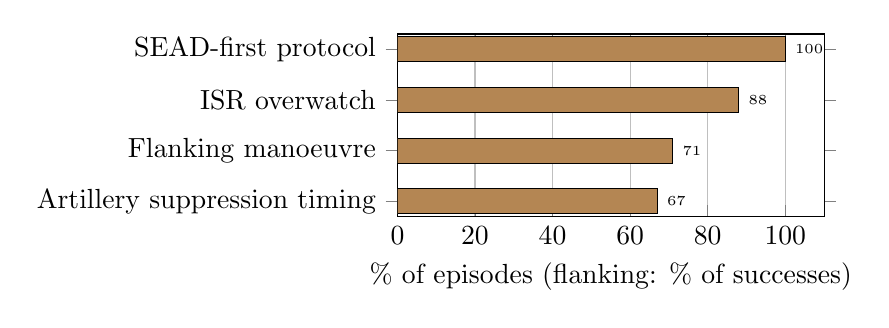
\begin{tikzpicture}\begin{axis}[xbar,width=7.0cm,height=3.9cm,symbolic y coords={Artillery suppression timing,Flanking manoeuvre,ISR overwatch,SEAD-first protocol},ytick=data,xmin=0,xmax=110,bar width=9pt,nodes near coords,nodes near coords style={font=\fontsize{5.5}{6}\selectfont},xlabel={\% of episodes (flanking: \% of successes)},xmajorgrids]
\addplot[fill=AccentCol!75]coordinates{(67,Artillery suppression timing)(71,Flanking manoeuvre)(88,ISR overwatch)(100,SEAD-first protocol)};
\end{axis}\end{tikzpicture}}
\sm{A fifth tactic, bounding advance, was also identified (frequency not reported).}
\column{0.46\textwidth}
\begin{tl}\item \textbf{SEAD-first (100\%):} SAM is the existential threat; any episode with an active SAM fails often\item \textbf{ISR overwatch (88\%):} drones take high-ground vantage points covering ground units' blind spots --- learned geometric coverage\item \textbf{Flanking (71\% of successes):} infantry distracts frontally while armour flanks --- never explicitly rewarded; it emerged from the joint value gradient\item \textbf{Artillery timing (67\%):} fires during the flanking move\end{tl}
\begin{rbox}\scriptsize\textbf{Implication for doctrine:} MARL rediscovers valid doctrine and may reveal NEW coordination patterns; expert review of replay logs is itself a source of tactical insight.\end{rbox}
\end{columns}
\end{frame}

\sect{7. Comparison \& Safety}
\begin{frame}{Algorithm Comparison --- All MARL Methods vs the Human Expert Team}
\figc{2.7cm}{\scriptsize\renewcommand{\arraystretch}{1.12}\begin{tabular}{llccccl}\toprule\textbf{Method}&\textbf{Type}&\textbf{Success}&\textbf{Casualties}&\textbf{Turns}&\textbf{Train eps}&\textbf{Key strength}\\\midrule IQL (independent Q)&single-agent$\times$6&58.3\%&2.8&44.1&100K&baseline; ignores structure\\QMIX&value CTDE&74.1\%&1.8&38.2&200K&monotonic mix; greedy decentralised\\MADDPG&actor--critic CTDE&79.2\%&1.6&35.8&250K&per-agent critics; continuous\\MAPPO&PG CTDE&82.4\%&1.2&33.7&150K&shared params; best without comms\\\rowcolor{ISSAgrn!20}\textbf{CommsMAPPO}&PG + comms&\textbf{88.1\%}&\textbf{0.9}&\textbf{29.4}&180K&emergent language\\Human expert team&human&81.3\%&1.6&41.8&---&benchmark (with comms)\\\bottomrule\end{tabular}}
\begin{columns}[T]
\column{0.50\textwidth}
\figc{2.5cm}{\bars{100}{1.7}{1.15}{IQL/58.3/ISSAred,QMIX/74.1/ISSAblue,MADDPG/79.2/violet,MAPPO/82.4/AccentCol,Comms/88.1/ISSAgrn,Human/81.3/ISSAgrey}}
\column{0.48\textwidth}
\begin{rbox}\scriptsize\textbf{Takeaways:} ignoring multi-agent structure (IQL, 58.3\%) is deeply costly; MAPPO matches or slightly exceeds the human team; learned communication adds a further $\sim$6 points.\end{rbox}
\end{columns}
\end{frame}

\begin{frame}{When to Use Which --- and a MARL Safety Warning}
\begin{columns}[T]
\column{0.50\textwidth}
\begin{cbox}[ISSAblue]{QMIX}\scriptsize Purely cooperative; discrete actions; communication-denied; interpretable per-agent Q-values; off-policy sample efficiency. (Note: MAPPO still scored higher without comms in this study.)\end{cbox}
\begin{cbox}[AccentCol]{MAPPO}\scriptsize Large teams; heterogeneous agents; mixed tasks --- the most robust choice overall.\end{cbox}
\begin{cbox}[ISSAred]{MADDPG}\scriptsize Continuous actions; mixed competitive settings.\end{cbox}
\column{0.48\textwidth}
\begin{wbox}\scriptsize\textbf{MARL safety warning --- emergent behaviours are UNPREDICTABLE.} In some runs agents learned to conserve ammunition by NOT FIRING: locally rational under the reward, tactically bad. Deployment needs extensive red-teaming.\end{wbox}
\figc{2.4cm}{\begin{tikzpicture}\node[ndG,text width=2.4cm](a)at(0,0){intended: suppress the enemy};\node[ndR,text width=2.4cm](b)at(3.4,0){learned: hold fire to save ammo penalty};\draw[bigarr](a)--node[above,font=\tiny]{reward}(b);\node[lab]at(1.7,-0.9){the agent optimises what you reward, not what you meant};\end{tikzpicture}}
\end{columns}
\end{frame}

\sect{8. Autonomous Platforms}
\begin{frame}{Autonomous Combat Platforms --- Levels of Autonomy}
\begin{columns}[T]
\column{0.52\textwidth}
\figc{3.5cm}{\begin{tikzpicture}
\foreach \i/\t/\d/\cl in {1/Level 1 --- human-operated/full human control; AI assists targeting/ISSAgrn!35,2/Level 2 --- human-on-the-loop/AI nominates; human approves each action/ISSAgrn!20,3/Level 3 --- human-out-of-the-loop (LAWS)/engages without per-action approval; contested under IHL/ISSAamb!35,4/Level 4 --- fully autonomous/seeks; decides; engages for hours or days; prohibited in most militaries/ISSAred!30}{\node[anchor=west,draw=ISSAnavy,fill=\cl,minimum height=0.72cm,minimum width={4.2cm+\i*0.8cm},text width={4.0cm+\i*0.8cm},align=left,font=\fontsize{6.2}{7.2}\selectfont,inner sep=2pt]at(0,\i*0.85){\textbf{\t}\\\d};}
\end{tikzpicture}}
\sm{Illustrative ladder after DoD / UK MoD style frameworks.}
\column{0.46\textwidth}
\begin{cbox}[ISSAnavy]{Examples}\scriptsize L1: drone with AI camera assist. L2: \textbf{MAPPO advisory mode} --- 6 agents each recommend an action and a human approves (this course). L3: a loitering munition with target criteria; or QMIX in a comms-contested environment. L4: long-duration independent missions.\end{cbox}
\begin{rbox}\scriptsize\textbf{Level 2 is practical, legally reviewable and deployable now.} Every step up the ladder transfers judgement from accountable humans to a policy that was optimised in simulation.\end{rbox}
\end{columns}
\end{frame}

\begin{frame}{Manned--Unmanned Teaming (MUM-T) --- and the Ethical Bright Line}
\begin{columns}[T]
\column{0.50\textwidth}
\figc{2.6cm}{\begin{tikzpicture}
\node[ndN,minimum width=2.6cm,minimum height=0.8cm](p)at(0,0){human pilot\\\sm{objectives, threat priorities, ROE}};
\foreach \i/\x in {1/-1.8,2/0,3/1.8}{\node[ndA,minimum width=1.3cm](w\i)at(\x,-1.6){UAV \i\\\sm{MAPPO policy}};\draw[arr,<->](p)--(w\i);}
\node[lab]at(0,-2.4){datalink $\le$2 s latency; policy pre-trained on the ground, updated overnight};
\end{tikzpicture}}
\begin{cbox}[ISSAnavy]{ROE as reward shaping}\scriptsize The human provides waypoints, threat priorities and ROE; MAPPO encodes them as penalties: $r_{\text{ROE}}$ for engaging non-combatants, $r_{\text{prop}}$ for disproportionate engagement. Agents optimise the mission inside these constraints.\end{cbox}
\column{0.48\textwidth}
\begin{cbox}[ISSAamb]{Open challenges}\scriptsize \textcircled{\tiny1} trust calibration: when to override the agent; \textcircled{\tiny2} adversarial robustness: OPFOR exploiting learned patterns; \textcircled{\tiny3} accountability: who is responsible for an AI action?; \textcircled{\tiny4} sim-to-real transfer.\end{cbox}
\begin{wbox}\scriptsize\textbf{Ethical bright line:} MARL for ADVISORY and PLANNING purposes is current best practice. Autonomous lethal engagement (Level 3+) needs legal clarity under IHL on meaningful human control. This course treats MARL as decision support --- \textbf{the human remains the decision-maker for lethal force.}\end{wbox}
\begin{ibox}\scriptsize A penalty term is not a legal safeguard: reward shaping makes violations \emph{less likely}, not impossible. Human approval provides the guarantee.\end{ibox}
\end{columns}
\end{frame}

\sect{9. Across Disciplines}
\begin{frame}{Multi-Agent Systems Across the Disciplines}
\subhead{Coordination without a central controller is everywhere in nature, engineering and war}
\figc{5.0cm}{\begin{tikzpicture}
\tikzset{G/.style={nd,text width=4.75cm,align=left,minimum height=2.3cm,font=\fontsize{6.9}{8.2}\selectfont,inner sep=3pt}}
\node[G,draw=ISSAgrn,fill=ISSAgrn!7]at(-5,1.25){\textbf{\textcolor{ISSAgrn}{BIOLOGY}}\\Ants coordinate through pheromone trails left in the environment (stigmergy, Grass\'e 1959); ant colony optimisation (Dorigo, 1992) borrows the idea.\\\textbf{Defence:} decentralised route planning for swarms that cannot talk directly.};
\node[G,draw=ISSAamb,fill=ISSAyell!45]at(0,1.25){\textbf{\textcolor{ISSAamb!80!black}{STATISTICS / GAME THEORY}}\\Nash equilibrium (1950); Axelrod's iterated prisoner's-dilemma tournaments (1980s) showed tit-for-tat cooperation emerging between self-interested players.\\\textbf{Defence:} deterrence, escalation and coalition behaviour in strategic wargames.};
\node[G,draw=violet,fill=violet!7]at(5,1.25){\textbf{\textcolor{violet}{PSYCHOLOGY}}\\Social loafing: individuals pull less hard on a rope when pulling in a group (Ringelmann; Lat\'ane et al., 1979) --- the human free-rider problem.\\\textbf{MARL twin:} equal reward splits teach agents to coast; COMA-style credit fixes it.};
\node[G,draw=ISSAblue,fill=ISSAblue!7]at(-5,-1.25){\textbf{\textcolor{ISSAblue}{AERONAUTICS}}\\TCAS coordinates two aircraft (one climbs, one descends). At \"Uberlingen (2002) one crew followed a controller's contrary instruction and the aircraft collided.\\\textbf{Defence:} in MUM-T, authority between human and machine must be unambiguous.};
\node[G,draw=ISSAred,fill=ISSAred!6]at(0,-1.25){\textbf{\textcolor{ISSAred}{MILITARY DOCTRINE}}\\Mission command (\textit{Auftragstaktik}): commanders share intent centrally; subordinates act on local judgement when communications fail.\\\textbf{MARL twin:} this is CTDE --- centralised training, decentralised execution.};
\node[G,draw=AccentCol,fill=AccentCol!8]at(5,-1.25){\textbf{\textcolor{AccentCol}{GAMES \& WARGAMING}}\\AlphaStar reached Grandmaster level in StarCraft II by training a \emph{league} of agents against each other (Vinyals et al., \textit{Nature}, 2019) to avoid exploitable strategies.\\\textbf{Use:} league self-play for robust OPFOR agents.};
\end{tikzpicture}}
\begin{ibox}\scriptsize\textbf{Common thread:} shared intent plus local action scales; unclear credit or authority breaks teams of people and agents alike.\end{ibox}
\end{frame}

\sect{10. Summary}
\begin{frame}{Lecture 8 Summary --- From CTDE to Emergent Combined-Arms Tactics}
\figc{4.9cm}{\begin{tikzpicture}
\tikzset{K/.style={nd,text width=3.6cm,align=left,minimum height=2.1cm,font=\fontsize{6.4}{7.6}\selectfont,inner sep=3pt}}
\node[K,draw=ISSAblue,fill=ISSAblue!8]at(-4,1.2){\textbf{DEC-POMDP \& MARL}\\$N$ agents, partial observations, joint reward; non-stationarity is the core challenge; mixed coop.--competitive is the norm.\\\textbf{Foundation}};
\node[K,draw=ISSAgrn,fill=ISSAgrn!8]at(0,1.2){\textbf{CTDE}\\Train centralised, execute decentralised; plan rehearsal $\to$ radio silence; coordination without field comms.\\\textbf{Dominant} defence paradigm};
\node[K,draw=violet,fill=violet!8]at(4,1.2){\textbf{QMIX}\\Monotonic $Q_{\text{tot}}$; decentralised greedy execution; 74.1\%; off-policy, interpretable.\\\textbf{Use:} cooperative, comms-denied};
\node[K,draw=AccentCol,fill=AccentCol!10]at(-4,-1.2){\textbf{MAPPO}\\Shared actor + centralised critic; 82.4\% vs human team 81.3\%; PPO stability.\\\textbf{Go-to} for cooperative MARL};
\node[K,draw=ISSAamb,fill=ISSAyell!40]at(0,-1.2){\textbf{EMERGENT TACTICS}\\SEAD-first, ISR overwatch, flanking, artillery timing --- all from reward; plus an emergent message code.\\\textbf{Validates} doctrine; reveals patterns};
\node[K,draw=ISSAred,fill=ISSAred!7]at(4,-1.2){\textbf{MUM-T \& LAWS ETHICS}\\Level 2 advisory is best practice; ROE as reward shaping; lethal autonomy unresolved under IHL.\\\textbf{Human} decides on lethal force};
\end{tikzpicture}}
\end{frame}

\begin{frame}{Looking Ahead --- Lecture 9: Culmination \& Revision}
\begin{columns}[T]
\column{0.50\textwidth}
\subhead{Lecture 9: putting the whole course together}
\begin{tl}\item Full course concept map\item Cross-lecture case-study threads revisited\item Integrated AI/ML pipeline for defence scenarios\item Common exam misconceptions\item Rapid-fire MCQ revision\item Key formula sheet\end{tl}
\begin{ibox}\scriptsize\textbf{Assignment 8} is released with this pack. \textbf{Lecture 10:} student project presentations and the final Q\&A panel.\end{ibox}
\column{0.48\textwidth}
\figc{3.2cm}{\begin{tikzpicture}\tikzset{B/.style={nd,minimum width=1.6cm,minimum height=0.6cm}}
\node[B,fill=ISSAgrn!15](s)at(0,1.2){Supervised\\\sm{L2--L3}};\node[B,fill=teal!15](u)at(2.2,1.2){Unsupervised\\\sm{L4--L5}};\node[B,fill=blue!10](r)at(4.4,1.2){RL / MARL\\\sm{L6--L8}};\node[ndC,minimum width=5.6cm](d)at(2.2,0){data quality \& interpretation (L1)};\node[ndN,minimum width=5.6cm](p)at(2.2,-1.0){integrated defence AI pipeline (L9)};
\draw[arr](s)--(d);\draw[arr](u)--(d);\draw[arr](r)--(d);\draw[arr](d)--(p);
\end{tikzpicture}}
\end{columns}
\end{frame}
\end{document}
